\section{Blockchain Patterns}
\subsection{Patterns Overview}
\begin{frame}{Patterns}
    \begin{itemize}
        \item Token template
        \item Policy contract
        \item Token registery
        \item Token swap
        \item Burned token
    \end{itemize}
    \begin{figure}
        \caption{Carboncoin Lifecycle}
        \centering
        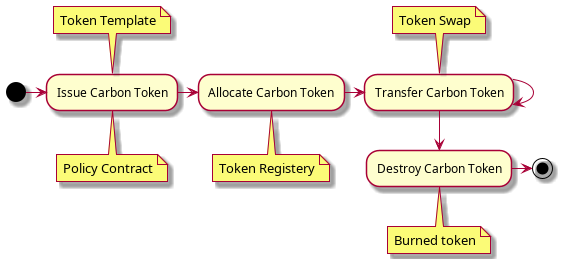
\includegraphics[height=0.5\textheight, width=0.6\linewidth,
            keepaspectratio]{photos/Token.png}
    \end{figure}
\end{frame}
\subsection{Policy Contract}
\begin{frame}{Policy Contract Pattern}
    \begin{itemize}
        \item All blockchain operations are bounded by policies which
              provide rules on how \textit{Carboncoin} can be used.
        \item Only producers with the \textit{producer} role can buy or
              sell \textit{Carboncoin}.
        \item A user can never sell more \textit{Carboncoin} than the amount
              contained inside their account.
        \item A user's \textit{X.509} certificate is required to perform write
              operations on the blockchain.
    \end{itemize}
\end{frame}
\subsection{Token Swap}
\begin{frame}{Token Swap Pattern}
    \begin{itemize}
        \item \textit{Carboncoin} can be swapped between users.
        \item Policies are attached when doing a swap:
              \begin{itemize}
                  \item Active offer is required.
                  \item Seller must have enough \textit{Carboncoin}.
                  \item The buyer must meet their open offer obligations first
                        before purchasing tokens.
              \end{itemize}
        \item The swap happens for only the \textit{Carboncoin} token.
    \end{itemize}
\end{frame}
\subsection{Burned Token}
\begin{frame}{Burned Token}
    \begin{itemize}
        \item A \textit{Carboncoin} is burned when a producer is required
              to pay for carbon production.
        \item \textit{Digital Physical Parity} exists between real carbon
              production and the carbon reputation in the market.
              \begin{itemize}
                  \item Certifiers play a signficant role in maintaining the
                        digital physical parity between carbon production and
                        carbon reputation.
              \end{itemize}
        \item Debts are recorded when a user does not have enough
              \textit{Carboncoin} to pay for carbon production. Debts can
              be paid at later dates.
    \end{itemize}
\end{frame}